In the Android environment, the term “activity” refers to the interaction entry point of Android applications for the end-user. Alternatively stated, an activity is a screen with a user interface. It would not be wrong to say that activity is the main component for building an Android application. Activities are represented by the “Activity” class of the Android Software Development Kit. Each activity of an Android application is implemented as a subclass of the Activity class \cite{9}. 

An Android application might have single or more activities. Oftentimes an Android application consists of a set of activities. An activity can start and finish another activity which means activities are also responsible for the navigation within the application. An activity can even start another Android application from the device. Activities within an app provide a strong user experience together. Since the activities of an Android application can affect each other and each activity has its own lifecycle, this situation has an important impact on the maintainability of the Android applications. Thus activity lifecycle should definitely be taken into account when developing Android applications. During the lifetime of activities, some actions should be taken and some methods should be called depending on the situation. Some of the important ones of these situations are covered in the upcoming sections but before discussing these, it is important to understand the activity lifecycle. The figure below is an illustration of the activity lifecycle and it presents the activity lifecycle methods. 

\begin{figure}[ht!]
    \centering
    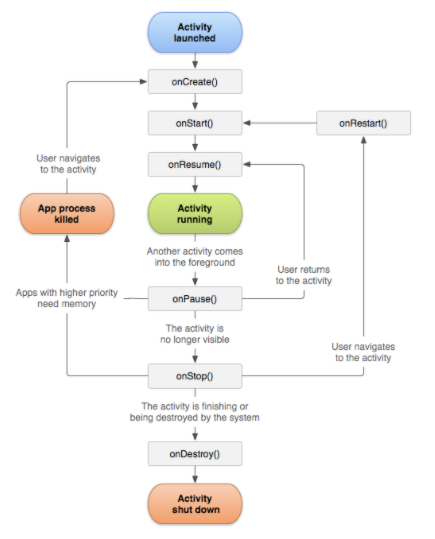
\includegraphics[scale=0.7]{figures/activity_lifecycle.png}
    \caption{Android activity lifecycle \protect\cite{9}}
    \label{fig:android_activity_life_cycle}
\end{figure}

Users navigate between the different Android applications and/or navigate within screens of an Android application. During this navigation instances of activities are created, destroyed, or put into different states of the activity lifecycle. The Activity class from the Android SDK offers several different callback methods that enable the activity to recognize the state changes. Those methods are called activity lifecycle callback methods. With the help of these callback methods, developers can decide how activities behave during state changes. Proper usage of the activity lifecycle callback methods helps developers to prevent situations such as using valuable Android system resources when users do not really need them, losing the users' last state when they leave an application, crashing when switching between different applications and losing the last state during device orientation changes. 

Improved knowledge of activity lifecycle callback methods is not only helpful for maintaining system resources, organizing the activity behaviors during the state changes, and preventing undesirable situations but also useful when it comes to integrating non-UI related components of an Android application to the activities. It is essential for using activities and these other components together in harmony with high efficiency. Good knowledge of these callback methods enables developers to be aware of when to add/release these non-UI related components to activities when building maintainable Android applications. Detailed explanations of the importance of the activity lifecycle methods and their functionality can be found in the Android developer guidelines \cite{9}.
